\documentclass[mathserif]{beamer}

\setbeamertemplate{frametitle}[default][center]%Centers the frame title.
\setbeamertemplate{navigation symbols}{}%Removes navigation symbols.
\setbeamertemplate{footline}{\raisebox{5pt}{\makebox[\paperwidth]{\hfill\makebox[10pt]{\scriptsize\insertframenumber}}}}
\setbeamertemplate{caption}[numbered]

\usepackage{amssymb,amsfonts,amsmath,latexsym,amsthm}
%\usepackage[usenames,dvipsnames]{color}
%\usepackage[]{graphicx}
%\usepackage[space]{grffile}
\usepackage{mathrsfs}   % fancy math font
% \usepackage[font=small,skip=0pt]{caption}
\usepackage[skip=0pt]{caption}
\usepackage{subcaption}
\usepackage{verbatim}
\usepackage{url}
\usepackage{bm}
\usepackage{dsfont}
\usepackage{extarrows}
\usepackage{multirow}
%\newcommand{\tth}   {\mbox{$\theta$}}
\newcommand{\thh}   {\mbox{$\theta$}}
\newcommand{\su}   {\mbox{$\sigma^2$}}
\newcommand{\so}   {\mbox{$\sigma_0^2$}}
\newcommand{\ko}   {\mbox{$\kappa_0$}}
\newcommand{\no}   {\mbox{$\nu_0$}}
\newcommand{\mo}   {\mbox{$\mu_0$}}
\newcommand{\ti}   {\mbox{$\tilde{x}$}}
\newcommand{\la}   {\mbox{$\lambda$}}
\newcommand{\bx}   {\mbox{$\bm{x}$}}
\newcommand{\bZ}   {\mbox{$\bm{Z}$}}
\newcommand{\bX}   {\mbox{$\bm{X}$}}
\newcommand{\bY}   {\mbox{$\bm{Y}$}}
\newcommand{\bA}   {\mbox{$\bm{A}$}}
\newcommand{\ba}   {\mbox{$\bm{a}$}}
\newcommand{\bb}   {\mbox{$\bm{b}$}}
\newcommand{\bt}   {\mbox{$\bm{t}$}}
\newcommand{\bz}   {\mbox{$\bm{z}$}}
\newcommand{\bw}   {\mbox{$\bm{w}$}}
\newcommand{\bbeta}   {\mbox{$\bm{\beta}$}}

\newcommand{\be}   {\mbox{$\bm{e}$}}
\newcommand{\bu}   {\mbox{$\bm{u}$}}
\newcommand{\bv}   {\mbox{$\bm{v}$}}
\newcommand{\sig}   {\mbox{$\Sigma$}}
\newcommand{\sigx}   {\mbox{$\Sigma_{XX}$}}
\newcommand{\sigxy}   {\mbox{$\Sigma_{XY}$}}
\newcommand{\tr}   {\mbox{$\text{tr}$}}
\newcommand{\ddet}   {\mbox{$\text{det}$}}
\newcommand\independent{\protect\mathpalette{\protect\independenT}{\perp}}
\def\independenT#1#2{\mathrel{\rlap{$#1#2$}\mkern2mu{#1#2}}}

\newcommand{\Expect}[1]{\ensuremath{\mathbf{E}\left[ #1 \right]}}
%\newcommand{\Var}[1]{\ensuremath{\mathrm{Var}\left[ #1 \right]}}
%\newcommand{\Cov}[1]{\ensuremath{\mathrm{Cov}\left[ #1 \right]}}
\newcommand{\MSE}{\ensuremath{\mathrm{MSE}}}
\newcommand{\RSS}{\ensuremath{\mathrm{RSS}}}
\newcommand{\Prob}[1]{\ensuremath{\mathrm{Pr}\left( #1 \right)}}
\newcommand{\ProbEst}[1]{\ensuremath{\widehat{\mathrm{Pr}}\left( #1 \right)}}
\DeclareMathOperator*{\argmin}{argmin} % thanks, wikipedia!
\DeclareMathOperator*{\argmax}{argmax} % thanks, wikipedia!
\DeclareMathOperator*{\sgn}{sgn} % thanks, wikipedia!

\newcommand{\lam}{\lambda}
\newcommand{\bmu}{\bm{\mu}}
%\newcommand{\bx}{\ensuremath{\mathbf{X}}}
\newcommand{\X}{\ensuremath{\mathbf{X}}}
\newcommand{\w}{\ensuremath{\mathbf{w}}}
\newcommand{\h}{\ensuremath{\mathbf{h}}}
\newcommand{\V}{\ensuremath{\mathbf{V}}}
%\newcommand{\tr}{\operatorname{tr}}

%\newcommand{\bx}{\ensuremath{\mathbf{X}}}
%\newcommand{\X}{\ensuremath{\mathbf{x}}}
%\newcommand{\w}{\ensuremath{\mathbf{w}}}
%\newcommand{\h}{\ensuremath{\mathbf{h}}}
%\newcommand{\V}{\ensuremath{\mathbf{v}}}
%\newcommand{\Cov}{\text{Cov}}
%\newcommand{\Var}{\text{Var}}

\DeclareMathOperator{\var}{Var}
\DeclareMathOperator{\cov}{Cov}
\newcommand{\Var}[1]{\ensuremath{\mathrm{Var}\left[ #1 \right]}}
\newcommand{\Cov}[1]{\ensuremath{\mathrm{Cov}\left[ #1 \right]}}


\newcommand{\indep}{\rotatebox{90}{\ensuremath{\models}}}
\newcommand{\notindep}{\not\hspace{-.05in}\indep}







\usepackage{float,bm}
\floatstyle{boxed}
\newfloat{code}{tp}{code}
\floatname{code}{Code Example}
%\newcommand{\tth}   {\mbox{$\theta$}}
\newcommand{\thh}   {\mbox{$\theta$}}
\newcommand{\su}   {\mbox{$\sigma^2$}}
\newcommand{\so}   {\mbox{$\sigma_0^2$}}
\newcommand{\ko}   {\mbox{$\kappa_0$}}
\newcommand{\no}   {\mbox{$\nu_0$}}
\newcommand{\mo}   {\mbox{$\mu_0$}}
\newcommand{\ti}   {\mbox{$\tilde{x}$}}
\newcommand{\la}   {\mbox{$\lambda$}}
\newcommand{\bx}   {\mbox{$\bm{x}$}}
\newcommand{\bZ}   {\mbox{$\bm{Z}$}}
\newcommand{\bX}   {\mbox{$\bm{X}$}}
\newcommand{\bY}   {\mbox{$\bm{Y}$}}
\newcommand{\bA}   {\mbox{$\bm{A}$}}
\newcommand{\ba}   {\mbox{$\bm{a}$}}
\newcommand{\bb}   {\mbox{$\bm{b}$}}
\newcommand{\bt}   {\mbox{$\bm{t}$}}
\newcommand{\bz}   {\mbox{$\bm{z}$}}
\newcommand{\bw}   {\mbox{$\bm{w}$}}
\newcommand{\bbeta}   {\mbox{$\bm{\beta}$}}

\newcommand{\be}   {\mbox{$\bm{e}$}}
\newcommand{\bu}   {\mbox{$\bm{u}$}}
\newcommand{\bv}   {\mbox{$\bm{v}$}}
\newcommand{\sig}   {\mbox{$\Sigma$}}
\newcommand{\sigx}   {\mbox{$\Sigma_{XX}$}}
\newcommand{\sigxy}   {\mbox{$\Sigma_{XY}$}}
\newcommand{\tr}   {\mbox{$\text{tr}$}}
\newcommand{\ddet}   {\mbox{$\text{det}$}}
\newcommand\independent{\protect\mathpalette{\protect\independenT}{\perp}}
\def\independenT#1#2{\mathrel{\rlap{$#1#2$}\mkern2mu{#1#2}}}

\newcommand{\Expect}[1]{\ensuremath{\mathbf{E}\left[ #1 \right]}}
%\newcommand{\Var}[1]{\ensuremath{\mathrm{Var}\left[ #1 \right]}}
%\newcommand{\Cov}[1]{\ensuremath{\mathrm{Cov}\left[ #1 \right]}}
\newcommand{\MSE}{\ensuremath{\mathrm{MSE}}}
\newcommand{\RSS}{\ensuremath{\mathrm{RSS}}}
\newcommand{\Prob}[1]{\ensuremath{\mathrm{Pr}\left( #1 \right)}}
\newcommand{\ProbEst}[1]{\ensuremath{\widehat{\mathrm{Pr}}\left( #1 \right)}}
\DeclareMathOperator*{\argmin}{argmin} % thanks, wikipedia!
\DeclareMathOperator*{\argmax}{argmax} % thanks, wikipedia!
\DeclareMathOperator*{\sgn}{sgn} % thanks, wikipedia!

\newcommand{\lam}{\lambda}
\newcommand{\bmu}{\bm{\mu}}
%\newcommand{\bx}{\ensuremath{\mathbf{X}}}
\newcommand{\X}{\ensuremath{\mathbf{X}}}
\newcommand{\w}{\ensuremath{\mathbf{w}}}
\newcommand{\h}{\ensuremath{\mathbf{h}}}
\newcommand{\V}{\ensuremath{\mathbf{V}}}
%\newcommand{\tr}{\operatorname{tr}}

%\newcommand{\bx}{\ensuremath{\mathbf{X}}}
%\newcommand{\X}{\ensuremath{\mathbf{x}}}
%\newcommand{\w}{\ensuremath{\mathbf{w}}}
%\newcommand{\h}{\ensuremath{\mathbf{h}}}
%\newcommand{\V}{\ensuremath{\mathbf{v}}}
%\newcommand{\Cov}{\text{Cov}}
%\newcommand{\Var}{\text{Var}}

\DeclareMathOperator{\var}{Var}
\DeclareMathOperator{\cov}{Cov}
\newcommand{\Var}[1]{\ensuremath{\mathrm{Var}\left[ #1 \right]}}
\newcommand{\Cov}[1]{\ensuremath{\mathrm{Cov}\left[ #1 \right]}}


\newcommand{\indep}{\rotatebox{90}{\ensuremath{\models}}}
\newcommand{\notindep}{\not\hspace{-.05in}\indep}






%\usepackage{fontspec}
%\setmainfont{Tahoma}

%\newcommand{\lam}{\lambda}
%\newcommand{\bmu}{\bm{\mu}}
%%\newcommand{\bx}{\ensuremath{\mathbf{X}}}
%\newcommand{\X}{\ensuremath{\mathbf{x}}}
%\newcommand{\w}{\ensuremath{\mathbf{w}}}
%\newcommand{\h}{\ensuremath{\mathbf{h}}}
%\newcommand{\V}{\ensuremath{\mathbf{v}}}
%\newcommand{\cov}{\text{Cov}}
%\newcommand{\var{\text{Var}}}

%\DeclareMathOperator{\var}{Var}
%\DeclareMathOperator{\cov}{Cov}

%\newcommand{\indep}{\rotatebox{90}{\ensuremath{\models}}}
%\newcommand{\notindep}{\not\hspace{-.05in}\indep}

\usepackage{graphicx} %The mode "LaTeX => PDF" allows the following formats: .jpg  .png  .pdf  .mps
\graphicspath{{./PresentationPictures/}} %Where the figures folder is located
\usepackage{listings}
\usepackage{media9}
\usepackage{movie15}
\addmediapath{./Movies/}

\newcommand{\beginbackup}{
   \newcounter{framenumbervorappendix}
   \setcounter{framenumbervorappendix}{\value{framenumber}}
}
\newcommand{\backupend}{
   \addtocounter{framenumbervorappendix}{-\value{framenumber}}
   \addtocounter{framenumber}{\value{framenumbervorappendix}} 
}


%\usepackage{algorithm2e}
\usepackage[ruled,lined]{algorithm2e}
\def\algorithmautorefname{Algorithm}
\SetKwIF{If}{ElseIf}{Else}{if}{then}{else if}{else}{endif}
%\usepackage{times}
%\usepackage[tbtags]{amsmath}
%\usepackage{amssymb}
\usepackage{amsfonts}
%\usepackage{slfortheorems}
\usepackage{epsfig}
\usepackage{graphicx}
%\usepackage[small]{caption}
%\usepackage[square]{natbib}
%\newcommand{\newblock}{}
%\bibpunct{(}{)}{;}{a}{}{,}
%\bibliographystyle{ims}
%\usepackage[letterpaper]{geometry}
%\usepackage{color}
%\setlength{\parindent}{0pt}

\usepackage{natbib}
\bibpunct{(}{)}{;}{a}{}{,}
%\usepackage{hyperref}

\DeclareMathOperator*{\Exp}{Exp}
\DeclareMathOperator*{\TExp}{TExp}
\DeclareMathOperator*{\Bernoulli}{Bernoulli}
\DeclareMathOperator*{\Beta}{Beta}
\DeclareMathOperator*{\Ga}{Gamma}
\DeclareMathOperator*{\TGamma}{TGamma}
\DeclareMathOperator*{\Poisson}{Poisson}
\DeclareMathOperator*{\Binomial}{Binomial}
\DeclareMathOperator*{\NormalGamma}{NormalGamma}
\DeclareMathOperator*{\InvGamma}{InvGamma}
\DeclareMathOperator*{\Cauchy}{Cauchy}
\DeclareMathOperator*{\Uniform}{Uniform}
\DeclareMathOperator*{\Gumbel}{Gumbel}
\DeclareMathOperator*{\Pareto}{Pareto}
\DeclareMathOperator*{\Mono}{Mono}
\DeclareMathOperator*{\Geometric}{Geometric}
\DeclareMathOperator*{\Wishart}{Wishart}

\newcommand{\N}{\mathcal{N}}

\newcommand{\R}{\mathbb{R}}
\newcommand{\Z}{\mathbb{Z}}
\newcommand{\E}{\mathbb{E}}
\renewcommand{\Pr}{\mathbb{P}}
\newcommand{\I}{\mathds{1}}
\newcommand{\V}{\mathbb{V}}

% Math operators
\DeclareMathOperator*{\diag}{diag}
\DeclareMathOperator*{\median}{median}
\DeclareMathOperator*{\Vol}{Vol}

% Miscellaneous commands
\newcommand{\iid}{\stackrel{\mathrm{iid}}{\sim}}
\newcommand{\matrixsmall}[1]{\bigl(\begin{smallmatrix}#1\end{smallmatrix} \bigr)}

\newcommand{\items}[1]{\begin{itemize} #1 \end{itemize}}

\newcommand{\todo}[1]{\emph{\textcolor{red}{(#1)}}}

\newcommand{\branch}[4]{
\left\{
	\begin{array}{ll}
		#1  & \mbox{if } #2 \\
		#3 & \mbox{if } #4
	\end{array}
\right.
}

% approximately proportional to
\def\app#1#2{%
  \mathrel{%
    \setbox0=\hbox{$#1\sim$}%
    \setbox2=\hbox{%
      \rlap{\hbox{$#1\propto$}}%
      \lower1.3\ht0\box0%
    }%
    \raise0.25\ht2\box2%
  }%
}
\def\approxprop{\mathpalette\app\relax}

\newcommand{\btheta}{{\bm\theta}}
\newcommand{\bbtheta}{{\pmb{\bm\theta}}}

%\usepackage{zref-savepos}
%
%\newcounter{restofframe}
%\newsavebox{\restofframebox}
%\newlength{\mylowermargin}
%\setlength{\mylowermargin}{2pt}
%
%\newenvironment{restofframe}{%
%    \par%\centering
%    \stepcounter{restofframe}%
%    \zsavepos{restofframe-\arabic{restofframe}-begin}%
%    \begin{lrbox}{\restofframebox}%
%}{%
%    \end{lrbox}%
%    \setkeys{Gin}{keepaspectratio}%
%    \raisebox{\dimexpr-\height+\ht\strutbox\relax}[0pt][0pt]{%
%    \resizebox*{!}{\dimexpr\zposy{restofframe-\arabic{restofframe}-begin}sp-\zposy{restofframe-\arabic{restofframe}-end}sp-\mylowermargin\relax}%
%        {\usebox{\restofframebox}}%
%    }%
%    \vskip0pt plus 1filll\relax
%    \mbox{\zsavepos{restofframe-\arabic{restofframe}-end}}%
%    \par
%}


\usepackage{tikz}
\usetikzlibrary{arrows}

%\usepackage[usenames,dvipsnames]{xcolor}
\usepackage{tkz-berge}
\usetikzlibrary{fit,shapes}

\usepackage{calc}
%%
%% The tikz package is used for doing the actual drawing.
%\usepackage{tikz}
%%
%% In order to be able to put arrowheads in the middle of directed edges, we need an extra library.
\usetikzlibrary{decorations.markings}
%%
%% The next line says how the "vertex" style of nodes should look: drawn as small circles.
\tikzstyle{vertex}=[circle, draw, inner sep=0pt, minimum size=6pt]
%%
%% Next, we make a \vertex command as a shorthand in place of \node[vertex} to get that style.
\newcommand{\vertex}{\node[vertex]}
%%
%% Finally, we declare a "counter", which is what LaTeX calls an integer variable, for use in
%% the calculations of angles for evenly spacing vertices in circular arrangements.
\newcounter{Angle}

\newtheoremstyle{example}
{\topsep} % space above
{\topsep} % space below
{} % body font
{} % indent
{\bf} % head font
{:} % punctuation between head and body
{0.5em} % space after head
{} % manually specify head
%{\thmname{#1}\thmnumber{ #2}\thmnote{:#3}} % manually specify head

\theoremstyle{example}
\newtheorem{ex}{Example}[section]

\newtheoremstyle{definition}
{\topsep} % space above
{\topsep} % space below
{} % body font
{} % indent
{\sc} % head font
{:} % punctuation between head and body
{0.5em} % space after head
{} % manually specify head
%{\thmname{#1}\thmnumber{ #2}\thmnote{:#3}} % manually specify head

\theoremstyle{definition}
\newtheorem{defn}{Definition}[section]

\theoremstyle{rem}
\newtheorem{rem}{Remark}[section]

\newtheoremstyle{theorem}
{\topsep} % space above
{\topsep} % space below
{} % body font
{} % indent
{\sc} % head font
{:} % punctuation between head and body
{0.5em} % space after head
{} % manually specify head
%{\thmname{#1}\thmnumber{ #2}\thmnote{:#3}} % manually specify head

\theoremstyle{theorm}
\newtheorem{thm}{Theorem}[section]



%%%to add in new counter for slides in beamer

%\setbeamertemplate{footline}{
%  \leavevmode%
%  \hbox{%
%  \begin{beamercolorbox}[wd=.333333\paperwidth,ht=2.25ex,dp=1ex,center]{author in head/foot}%
%    \usebeamerfont{author in head/foot}\insertshortauthor~~(\insertshortinstitute)
%  \end{beamercolorbox}%
%  \begin{beamercolorbox}[wd=.333333\paperwidth,ht=2.25ex,dp=1ex,center]{title in head/foot}%
%    \usebeamerfont{title in head/foot}\insertshorttitle
%  \end{beamercolorbox}%
%  \begin{beamercolorbox}[wd=.333333\paperwidth,ht=2.25ex,dp=1ex,right]{date in head/foot}%
%    \usebeamerfont{date in head/foot}\insertshortdate{}\hspace*{2em}
%    \insertframenumber{} \hspace*{2ex} % hier hat's sich ge�ndert
%  \end{beamercolorbox}}%
%  \vskip0pt%
%}



%%%%%

\newcommand*\oldmacro{}
\let\oldmacro\insertshortauthor
\renewcommand*\insertshortauthor{
  \leftskip=.3cm
\insertframenumber\,/\,\inserttotalframenumber\hfill\oldmacro}




%\excludecomment{notbeamer}
%\includecomment{beamer}



\title{The Multi Stage Gibbs Sampling}
\author{Rebecca C. Steorts \\ Bayesian Methods and Modern Statistics: STA 360/601}
\date{Module 8}

\begin{document}

\maketitle

\frame{
The generalization to more than two variables is straightforward. 

\vskip 1em

We cycle through the variables, sampling each from its conditional distributional given all the rest.}

\frame{
\frametitle{Three Stage GS}
Assume three random variables, with joint pmf or pdf: $p(x,y,z).$.
\vskip 1em
Set $x$, $y$, and $z$ to some values $(x_o,y_o,z_o)$.
\vskip 1em
Sample $x|y,z$, then $y|x,z$, then $z|x,y$, then $x|y,z$, and so on. More precisely,
\begin{enumerate}
\item[0.] Set $(x_0,y_0,z_0)$ to some starting value.
\item[1.] Sample $x_1\sim p(x|y_0,z_0)$. \\
          Sample $y_1\sim p(y|x_1,z_0)$. \\
          Sample $z_1\sim p(z|x_1,y_1)$. \\
\item[2.] Sample $x_2\sim p(x|y_1,z_1)$. \\
          Sample $y_2\sim p(y|x_2,z_1)$. \\
          Sample $z_2\sim p(z|x_2,y_2)$. \\
        $\vdots$
\end{enumerate}

}

\frame{
\frametitle{Multistage GS}

Assume $d$ random variables, with joint pmf or pdf $p(v^1,\ldots,v^d)$.
\vskip 1em
 At each iteration $(1, \ldots, M)$ of the algorithm, we sample from
\begin{align*}
v^1&\mid v^2,v^3,\ldots,v^d\\
v^2&\mid v^1,v^3,\ldots,v^d\\
&\vdots\\
v^d&\mid v^1,v^2,\ldots,v^{d-1}
\end{align*}
always using the most recent values of all the other variables. 
\vskip 1em
The conditional distribution of a variable given all of the others is referred to as the \emph{full conditional} in this context, and for brevity denoted $v^i|\cdots$.

}

\frame{
\frametitle{Example: Censored data}
In many real-world data sets, some of the data is either missing altogether or is partially obscured. 
%Gibbs sampling provides a method for dealing with these situations in a completely coherent Bayesian way, by sampling these missing variables along with the parameters. This also provides information about the values of the missing/obscured data.
\vskip 1em

One way in which data can be partially obscured is by \emph{censoring}, which means that we know a data point lies in some particular interval, but we don't get to observe it exactly. 

%\vskip 1em
%Censored data occurs very frequently in medical research such as clinical trials (since for instance, the researchers may lose contact with some of the patients).

}

\frame{
\frametitle{Medical data censoring}

6 patients participate in a cancer trial, however, patients 1, 2 and 4 leave the trial early.
Then we know when they leave the study, but we don't know information about them as the trial continues.

\begin{figure}
  \begin{center}
    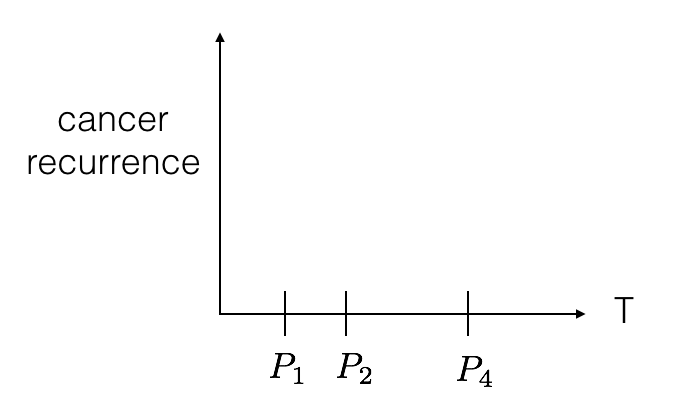
\includegraphics[width=0.5\textwidth]{censoring}
  \end{center}
  \caption{Example of censoring for medical data.}
\end{figure}\

This is a certain type of missing data.


}

\frame{
\frametitle{Heart Disease (Censoring) Example}
\begin{itemize}
\item Researchers are studying the length of life (lifetime) following a particular medical intervention, such as a new surgical treatment for heart disease.
\item The study consists of 12 patients.
\item The number of years before death for each is
$$3.4, 2.9, 1.2+, 1.4, 3.2, 1.8, 4.6, 1.7+, 2.0+, 1.4+, 2.8, 0.6+$$
where $x+$ indicates that the patient was alive after $x$ years, but the researchers lost contact with the patient at that point. 
\end{itemize}
%\item(Of
%course, there will always also be a control group, but let's focus on one group to keep things simple.) 




}

\frame{

Consider the following model:
\begin{align}
  &X_i = \branch{Z_i}{Z_i\leq c_i}{\ast}{Z_i > c_i.}\\
     &Z_1,\ldots,Z_n|\theta\,\iid\,\Ga(r,\theta)\\
    &\btheta\sim \Ga(a, b)
\end{align}
where $a$, $b$, and $r$ are known, and $\ast$ is a special value to indicate that censoring has occurred.  The interpretation is:
\begin{itemize}
\item $X_i$ is the observation
\begin{itemize}
\item if the lifetime is less than $c_i$ then we get to observe it ($X_i = Z_i$), 
\item otherwise
        all we know is the lifetime is greater than $c_i$ ($X_i = \ast$).
        \end{itemize}
    \item $\theta$ is the parameter of interest---the rate parameter for the lifetime distribution.
    \item $Z_i$ is the lifetime for patient $i$, however, this is not directly observed.
    \item $c_i$ is the censoring time for patient $i$, which is fixed, but known only if censoring occurs.
    \end{itemize}
}

\frame{
\frametitle{Gibbs saves us again!}
Straightforward approaches that are in closed form don't seem to work (think about these on your own). Instead we turn to GS. 
\vskip 1em


To sample from $p(\theta,z_{1:n}|x_{1:n})$, we cycle through each of the full conditional distributions,
\begin{align*}
\theta &\mid z_{1:n}, x_{1:n}\\
z_1 &\mid \theta, z_{2:n}, x_{1:n}\\
z_2 &\mid \theta, z_1,z_{3:n}, x_{1:n}\\
\vdots\\
z_n &\mid \theta, z_{1:n-1}, x_{1:n}
\end{align*}
sampling from each in turn, always conditioning on the most recent values of the other variables.
}

\frame{
Recall
\textcolor{blue}{
\begin{align*}
  &X_i = \branch{Z_i}{Z_i\leq c_i}{\ast}{Z_i > c_i.}\\
     &Z_1,\ldots,Z_n|\theta\,\iid\,\Ga(r,\theta)\\
    &\btheta\sim \Ga(a, b)
\end{align*}
}
The full conditionals are easy to calculate.
Let's start with $\theta|\cdots$
\begin{itemize}
\item Since $\theta \perp x_{1:n}\mid z_{1:n}$ (i.e., $\theta$ is conditionally independent of $x_{1:n}$ given $z_{1:n}$),
\begin{align}
p(\theta|\cdots) &= p(\theta|z_{1:n},x_{1:n}) = p(\theta|z_{1:n}) \\ &= \Ga\big(\theta\,\big\vert\, a+nr,\, b+\textstyle\sum_{i=1}^n z_i\big) 
\end{align}
using the fact that the prior on $\theta$ is conjugate. 
\end{itemize}
}

\frame{
Now let's move to $z?$
What happens here? This is the start of \textbf{Homework 5.}
\begin{enumerate}
\item Find the full conditional for $(z_i \mid \cdots$). 
%\begin{itemize}
%\item ($z_i|\cdots$) If $x_i\neq \ast$ then $z_i$ is forced to be equal to $x_i$. Otherwise,
%\begin{align*}
%p(z_i|\cdots) &= p(z_i|\theta,z_{(1:n) - i}, x_{1:n}) = p(z_i|\theta,x_i) \\
%&\underset{z_i}{\propto} p(x_i,z_i|\theta) = p(x_i|z_i) p(z_i|\theta)\\
%& =\I(z_i>c_i)\Ga(z_i\mid r,\theta)\\
%& \underset{z_i}{\propto} \TGamma(z_i\mid r,\theta,(c_i,\infty))
%\end{align*}
%where $\TGamma(z_i\mid r,\theta,S)$ is the truncated Gamma distribution---that is, the distribution of a $\Ga(r,\theta)$ random variable conditioned on being in the set $S$.
%\end{itemize}
\item Code up your own multi-stage GS in R. Be sure to use efficient functions. 
\item Use the censored data 
$$3.4, 2.9, 1.2+, 1.4, 3.2, 1.8, 4.6, 1.7+, 2.0+, 1.4+, 2.8, 0.6+$$
 and replicate such plots with explanations as in the Toy Example from Module 7. Specifically, give (a) give traceplots of all unknown paramaters from the G.S. (b) a running average plot,  (c) the estimated density of $\theta \mid \cdots $ and $z_9 \mid \cdots$. Be sure to give brief explanations of your results.
\end{enumerate}
}



%\frame{
%\frametitle{Multi-level modeling}
%\begin{itemize}
%\item Gibbs sampling is useful for models involving multiple levels.
%\item For instance, we may want to put a prior not only on the parameters, but also on the hyperparameters---that is, the parameters of the prior---this is called a \emph{hyperprior}. 
%\item This comes up particularly often when constructing \emph{hierarchical models}, that is, models in which there is a hierarchical structure to the relationships between the data, latent variables, and parameters.
%\end{itemize}
%
%
%}
%
%\frame{
%
%
%\begin{align*}
%& X_1,\ldots,X_n|\lambda_0,\mu,\lambda\,\sim\,\N(\mu,\lambda^{-1}).\\
%& \bm\mu|\lambda_0\,\sim\,\N(\mu_0,\lambda_0^{-1})\\
%& \bm\lambda_0 \sim \Ga(r,s)\\
%& \bm\lambda \sim \Ga(a,b)\\
%\end{align*}
%\begin{itemize}
%\item
%You might recognize that this is equivalent to putting a $t$-distribution prior on $\mu$. 
%\item Since the $t$-distribution is not a conjugate prior
%for the mean of Normally-distributed data, we would not be able to sample directly from $\mu|\lambda,x_{1:n}$.  
%\item However, we \textit{can}
%easily sample from $\mu|\lambda_0,\lambda,x_{1:n}$, and this is what we need for Gibbs sampling.
%\end{itemize}
%
%
%}
%
%\frame{
%\begin{itemize}
%    \item ($\lambda_0|\cdots$) Note $\lambda_0$ is conditionally independent of everything else given $\mu$, and thus
%        $$\bm\lambda_0|\mu,\lambda,x_{1:n} \,\sim\, \Ga\big(r+1/2,\,s+\tfrac{1}{2}(\mu-\mu_0)^2\big).$$
%    \item ($\mu|\cdots$) Since $\lambda_0$ is known, we are just in the usual situation for the semi-conjugate Normal
%        model without a hyperprior:
%        $$\bm\mu|\lambda_0,\lambda,x_{1:n}\, \sim \,\N(M,L^{-1})$$
%        where $L =\lambda_0+ n\lambda$ and $M =(\lambda_0\mu_0+\lambda\sum x_i)/(\lambda_0+ n\lambda)$.
%    \item ($\lambda|\cdots$) We are again just in the usual situation for the semi-conjugate Normal, and thus
%        $$\bm\lambda|\lambda_0,\mu,x_{1:n}\,\sim\,\Ga(A,B)$$
%        where $A = a + n/2$ and $B = n\hat\sigma^2 + n (\bar x-\mu)^2$.
%\end{itemize}
%Each iteration of Gibbs sampling proceeds by sampling from each of these, in turn.
%}
%
%\frame{
%\begin{itemize}
%\item We could just as easily put (semi-)conjugate priors on $\mu_0$ and $b$ as well (specifically, a Normal prior on $\mu_0$ and a Gamma prior on
%$b$), and include them as well in the Gibbs sampling algorithm.  
%\item Such hyperpriors essentially just make the prior
%less informative.
%\item However, when constructing hierarchical models involving multiple groups of datapoints, this approach can enable the
%``sharing of statistical strength'' across groups---roughly, using information learned from one group to help make inferences about the
%others.  
%\end{itemize}
%}




\end{document}